
\documentclass[thmsa,10pt]{article}
%%%%%%%%%%%%%%%%%%%%%%%%%%%%%%%%%%%%%%%%%%%%%%%%%%%%%%%%%%%%%%%%%%%%%%%%%%%%%%%%
%%%%%%%%%%%%%%%%%%%%%%%%%%%%%%%%%%%%%%%%%%%%\usepackage{amsmath}
\usepackage{url}
\usepackage{amssymb}
\usepackage{harvard}
\usepackage{graphicx}
\usepackage{amsmath}
\setlength{\oddsidemargin}{0.0in} \setlength{\evensidemargin}{0.0in}
\setlength{\textwidth}{6.5in} \setlength{\topmargin}{-0.2in}
\setlength{\textheight}{8.5in}
\renewcommand{\baselinestretch}{1.4}

%\input{tcilatex}
\begin{document}

%\pagenumbering{arabic} \pagestyle{plain}

\author{Shasha Wang}

\title{Research Project \\Economics 712}
%\date{}
\maketitle

\section{Partial Equilibrium}

\subsection{Agent's Problem}
The agent's Bellman equation is:
\begin{eqnarray}
v(a,y) &=& \max_{a^\prime,c} u(c)+\beta E_{y^\prime|y} v(a^\prime,y^\prime) \notag\\
s.t. && c+a^\prime = y+(1+r)a \notag
\end{eqnarray}

The stochastic Euler equation is:
\begin{equation}
u^\prime(c) = \beta (1+r)E_{y^\prime|y}  u^\prime(c^\prime) \notag
\end{equation}

\subsection{Infinite Horizon Results}

I use the following parameterization.
\begin{table}
\caption{Parameter Values}
\begin{center}
\begin{tabular}{l|c}
  \hline
  parameter &value\\
\hline
  CRRA &  1 \\
  Persistence of income shocks &  0.8 \\
  Discount rate & 0.04 \\
  Interest rate & 0.02 \\
  Borrowing limit & 0 \\
  \hline
\end{tabular}
\end{center}
\label{tab:param}
\end{table}

I consider both a low income shock case (variance=0.2) and a high income shock case (variance=0.4). Below I plot the value functions, policy function and average paths of consumption and asset holding for the first 61 periods of simulation.
\begin{figure}[h!]
\centering
\caption{Value Functions}
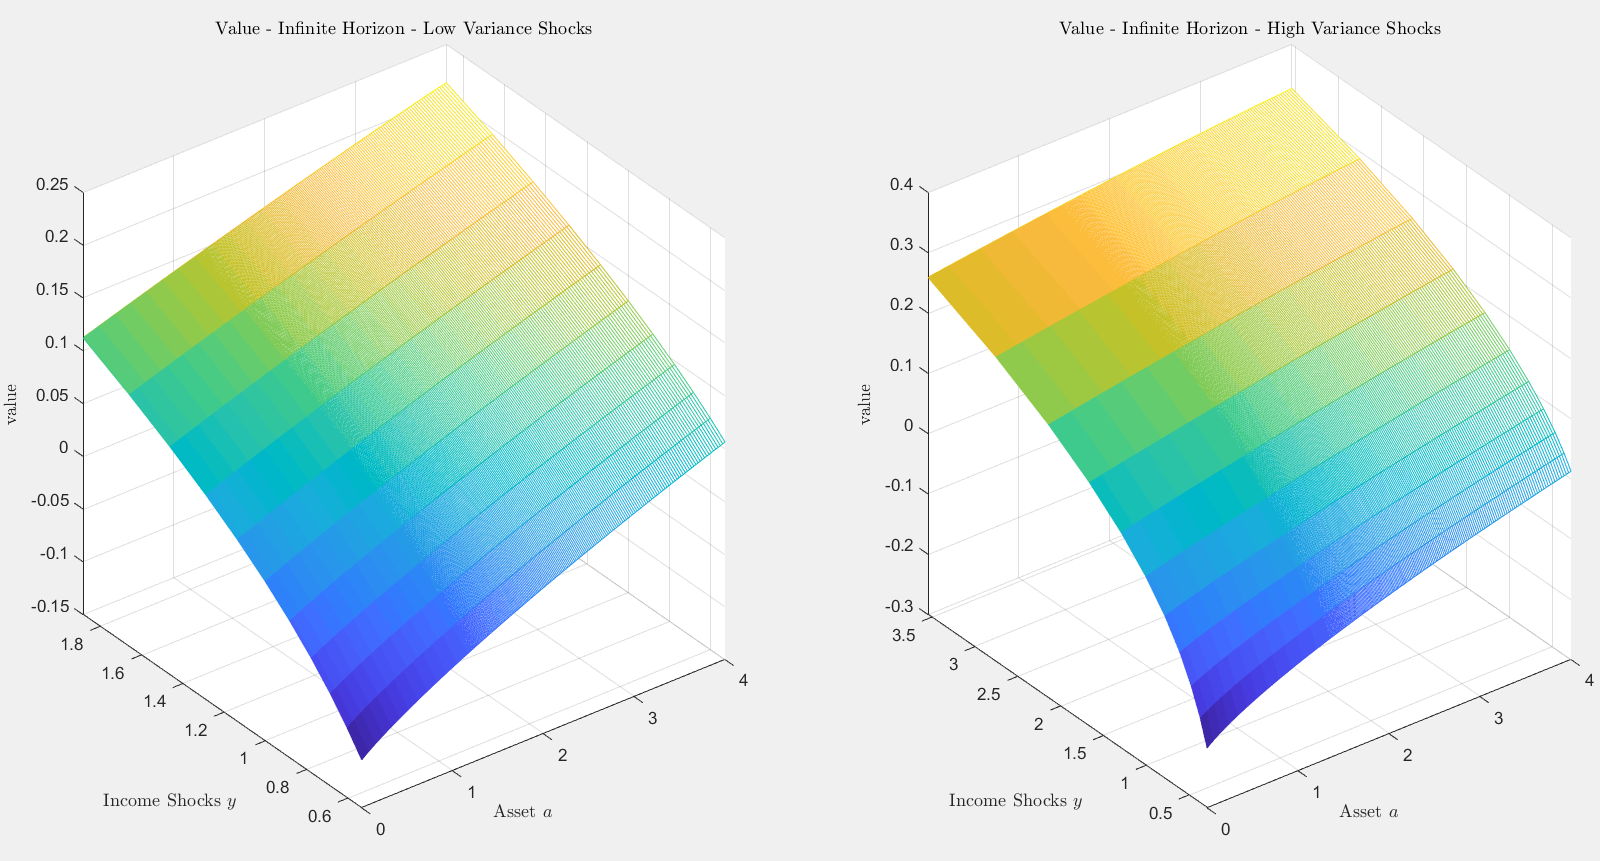
\includegraphics[width=12cm]{./figs/value}
\end{figure}
\begin{figure}[h!]
\centering
\caption{Consumption Policy Functions}
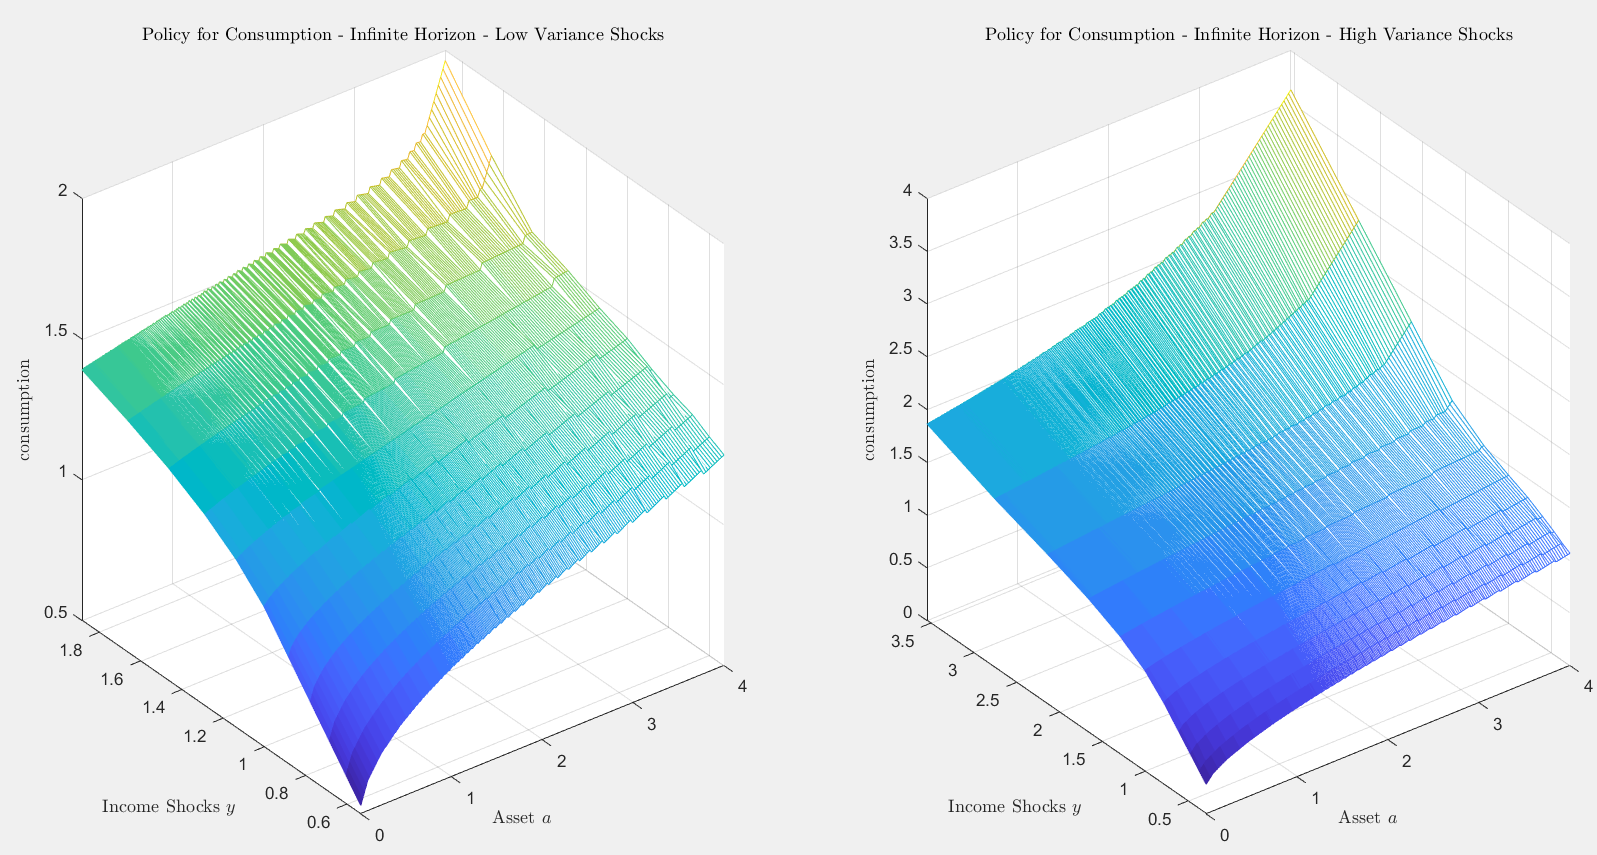
\includegraphics[width=12cm]{./figs/consumption}
\end{figure}
\begin{figure}[h!]
\centering
\caption{Asset Policy Functions}
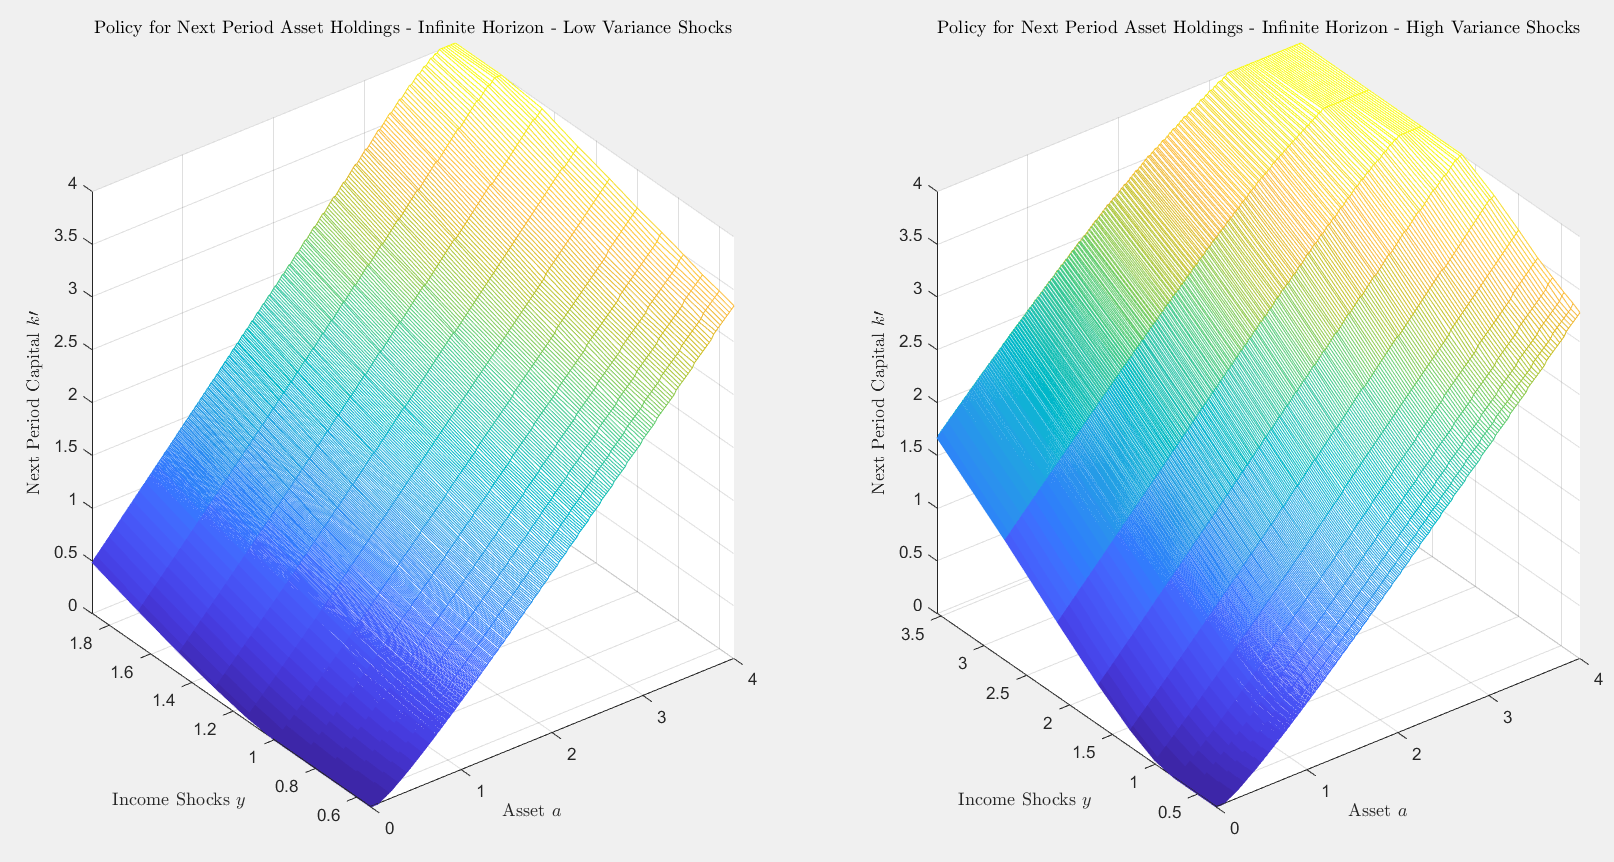
\includegraphics[width=12cm]{./figs/asset}
\end{figure}
\begin{figure}[h!]
\centering
\caption{Average Paths From Simulation}
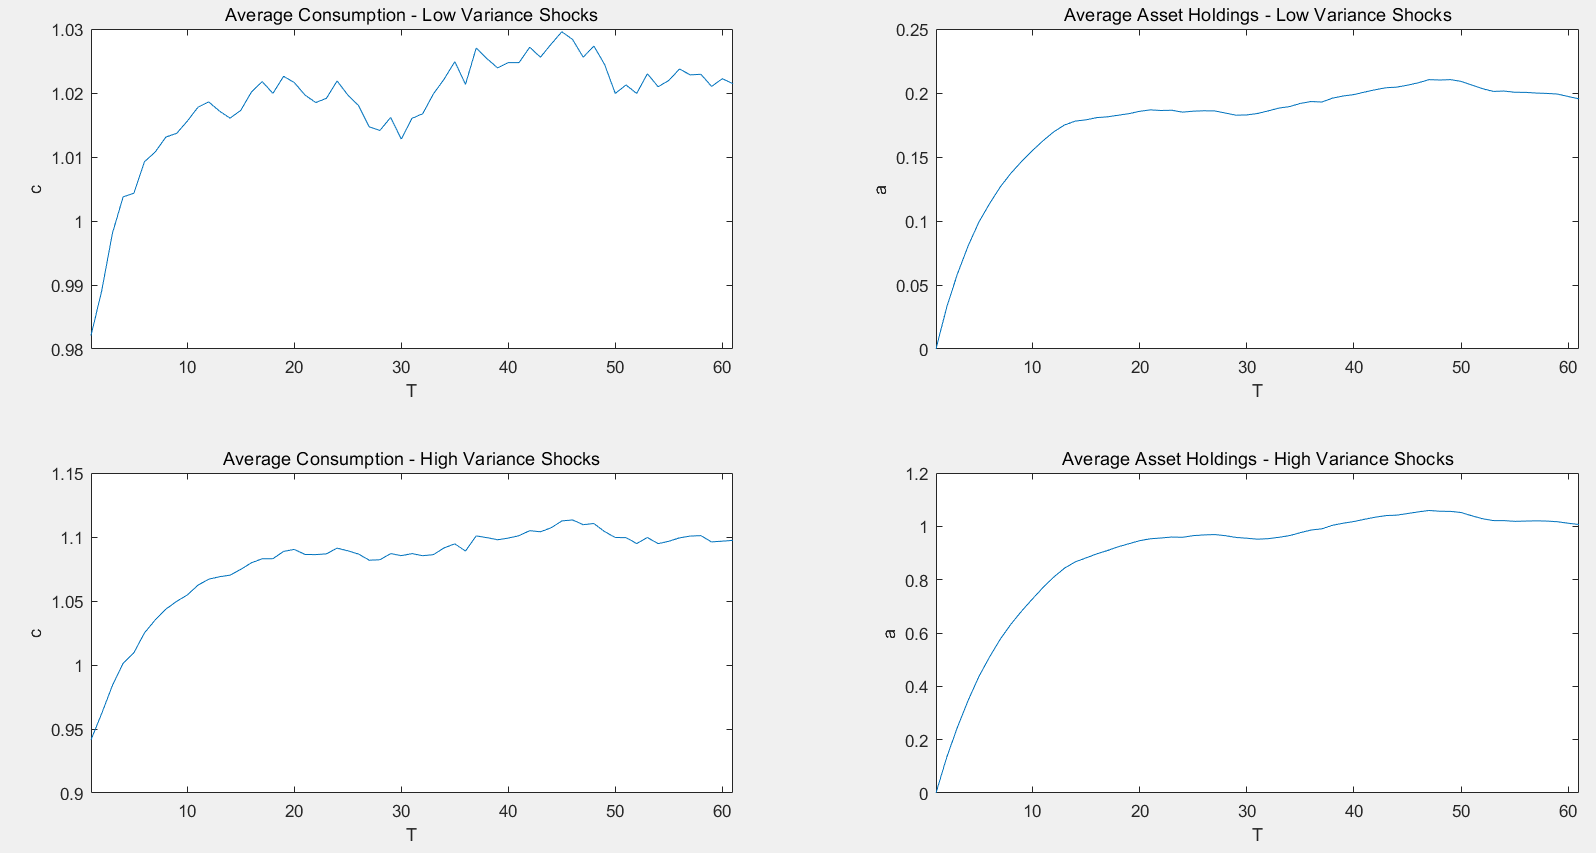
\includegraphics[width=12cm]{./figs/simulation}
\end{figure}

From these figures, it is obvious that, given a larger variance of income shocks, the agents accumulate more assets due to the stronger precautionary saving needs. As a results, 
the consumption level is also higher as the economy converges to the steady state.  

\newpage
\subsection{Finite Horizon Results}
Figure~\ref{fig:consumptionT} shows consumption functions from the finite horizon model with the same parameterization as in Table~\ref{tab:param}. Comparing consumption function at age 55 to the consumption function at age 1, it is clear that the former has a higher consumption level. This is because the agents need to build up a good stock of wealth to buffer against income shocks when they are young.
consumption level is higher 
\begin{figure}[h!]
\centering
\caption{Consumption Function From Finite Horizon Model (T=60)}
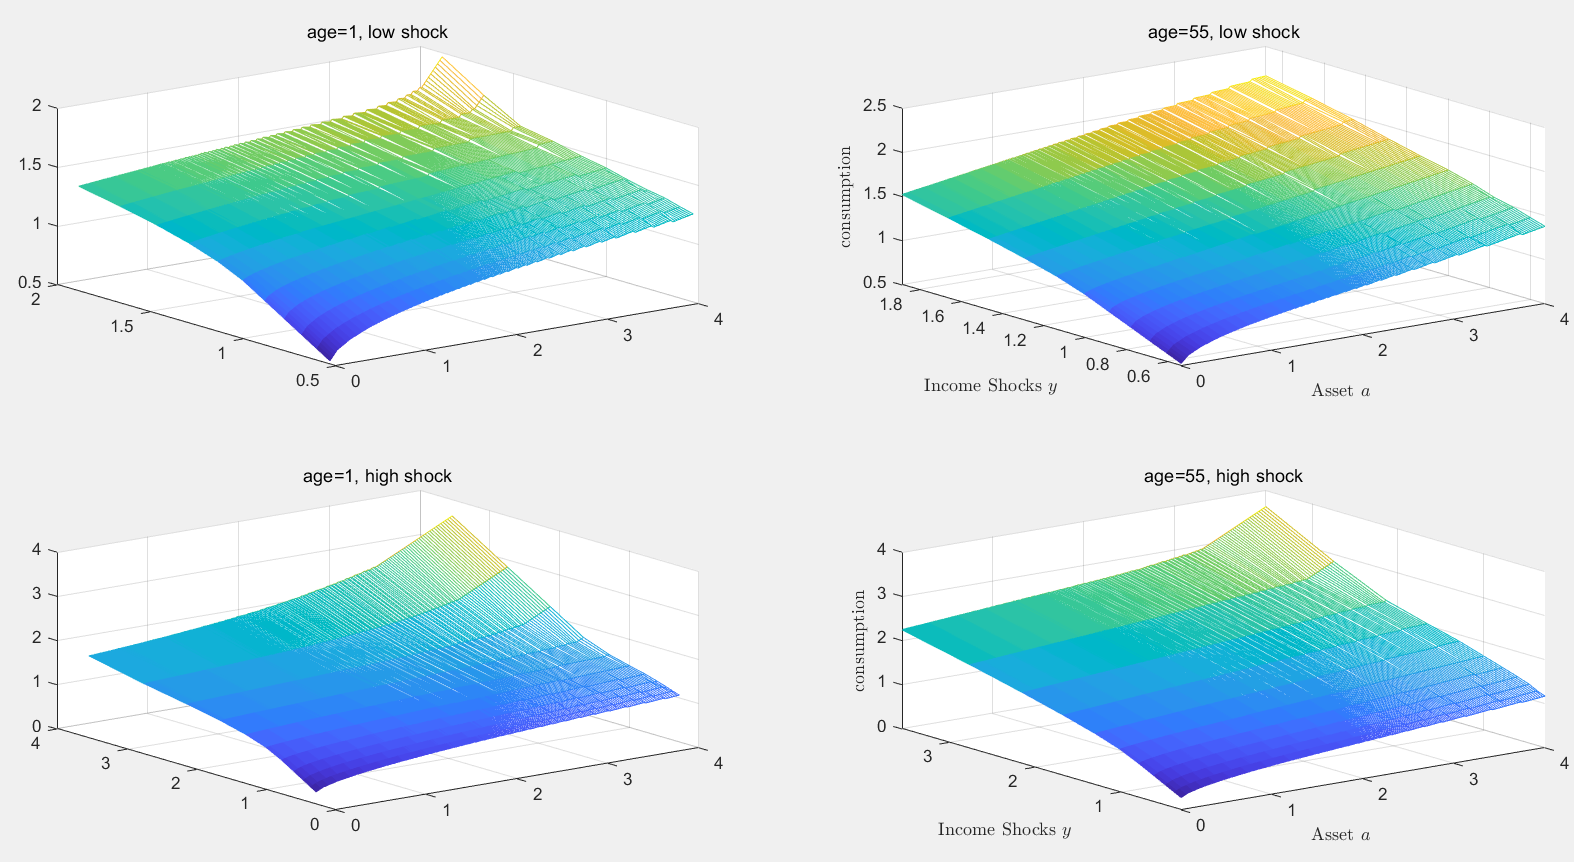
\includegraphics[width=12cm]{./figs/consumptionT}
\label{fig:consumptionT}
\end{figure}


\subsection{Consumption Profiles}
For question 6, I plot the average age profiles of consumption in Figure~\ref{fig:consprof} (left panel). The profiles are not hump-shaped. The agents tend to consume more as they approach the terminal period. This is understandable because the need to have a large stock of precautionary saving gets lower as the agents get closer to period T. I try different discount rates, borrowing constraints, and risk aversion, the consumption profile is not hump-shaped in each of these experiments. 

To substantiate my argument that agents have weaker precautionary motives, I also plot the age profile of asset holdings (right panel). The agents run down asset quickly in the last 10 years of life, which is consistent the quick rise of consumption during the same periods of life. 

\begin{figure}[h!]
\centering
\caption{Average Age Profiles of Consumption and Asset From Finite Horizon Model (T=60)}
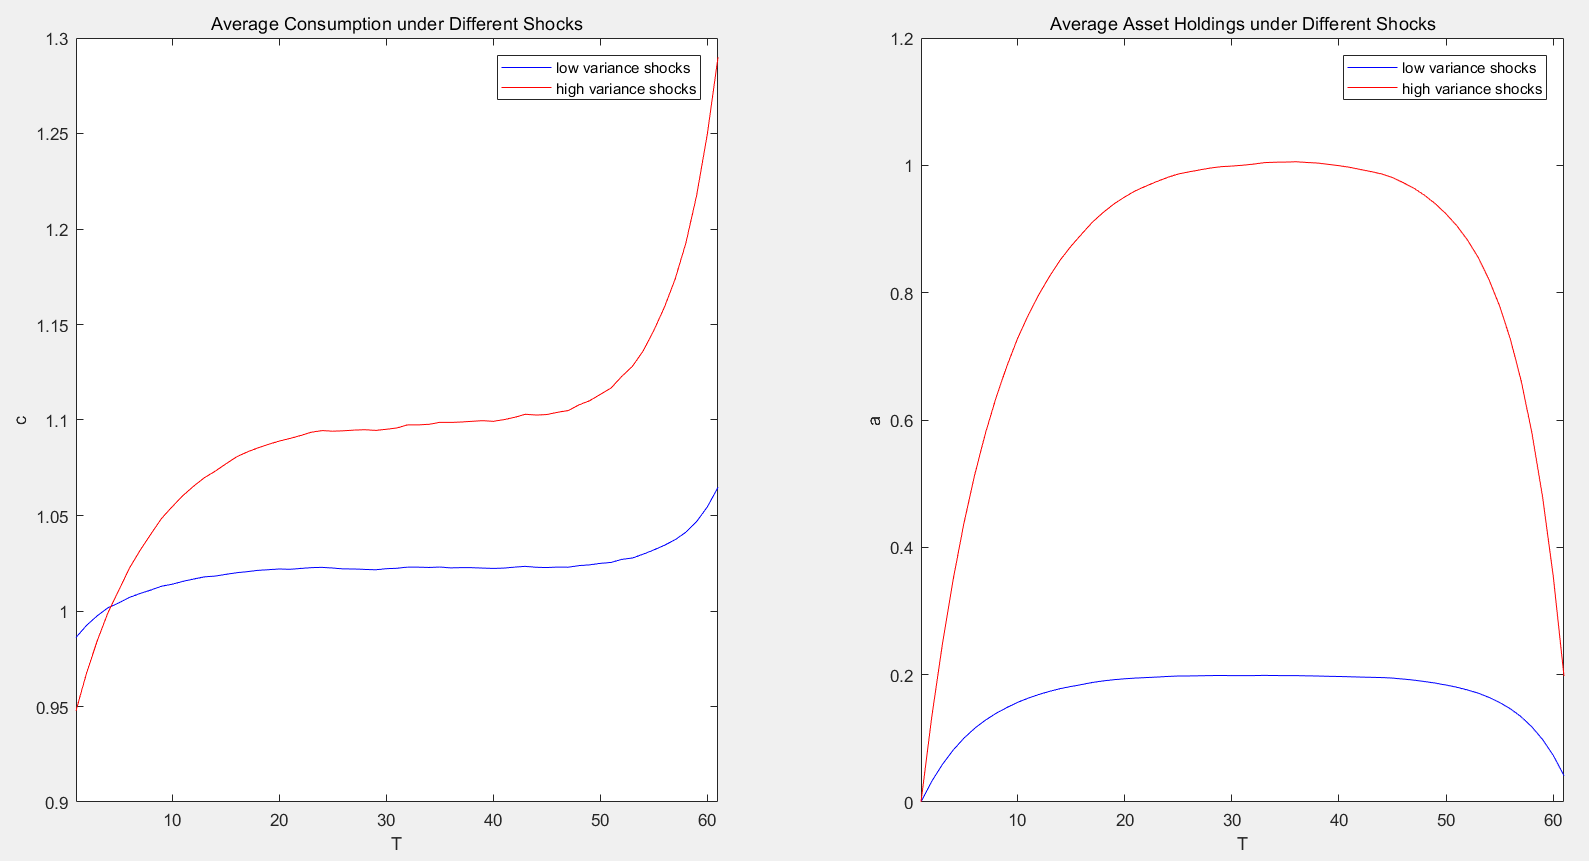
\includegraphics[width=12cm]{./figs/simulationT}
\label{fig:consprof}
\end{figure}


\subsection{Hump-Shaped Consumption Profiles}
For question 7, my result is reported in Figure~\ref{fig:hump}. The solid line shows the consumption profile from the model with high income shocks, assuming that an agent can borrow up to 5\% of its natural borrowing limit. The profile is hump-shaped, very different from the profiles in Figure~\ref{fig:consprof}.

\begin{figure}[h!]
\centering
\caption{Average Age Profiles (data vs model with hump-shaped income profile)}
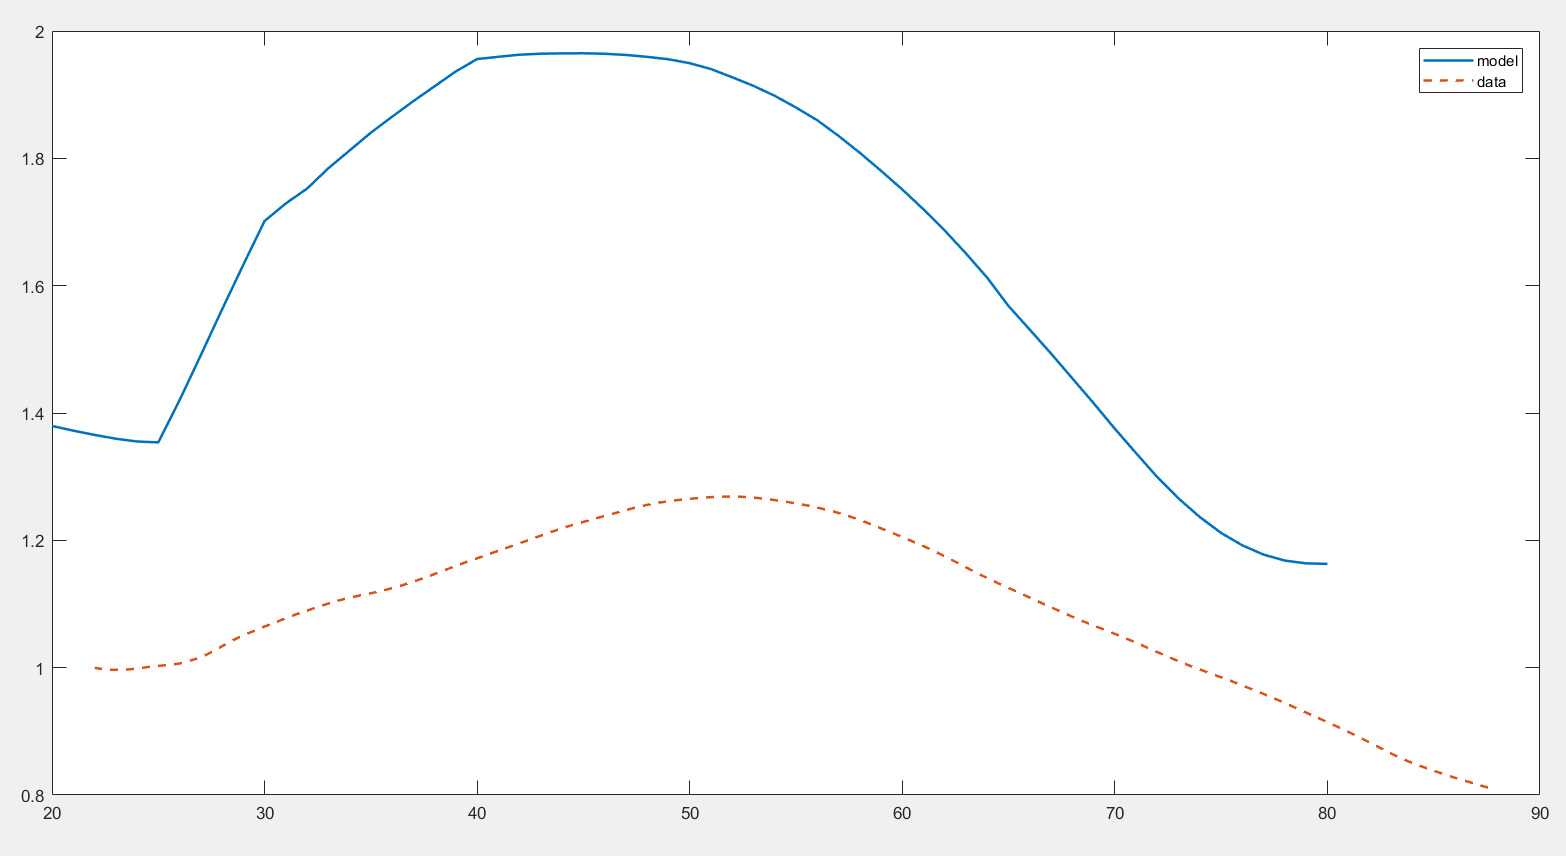
\includegraphics[width=9cm]{./figs/hump}
\label{fig:hump}
\end{figure}

For question 8, the comparison is presented in Figure~\ref{fig:hump}. Consumption level is higher from the model because the average income is larger than one in the model. The shape of consumption profile from the model is similar to that in the data. I find the shape is very sensitive to the borrowing limit. It is also sensitive to the discount rate and the degree of risk aversion. Adjusting these parameters can bring the two shapes closers. 


\subsection{Consumption Insurance}

I analyze consumption insurance based on the finite horizon model. Figure~\ref{fig:conins} reports consumption insurance coefficient by age and persistence of income shocks. 
The degree of consumption insurance is significantly larger when the income shock is less persistent, because low-persistence shocks can be easily insured away by assets. 
The degree of consumption insurance also depends on age. It peaks at age 65 which the age of retirement with the highest level of assets. After retirement, the agent runs down
asset, thus the agent's ability to insure against income shock is lower, and the degree of consumption insurance is also lower.

\begin{figure}[h!]
\centering
\caption{Consumption Insurance by Age and Persistence of Income Shocks)}
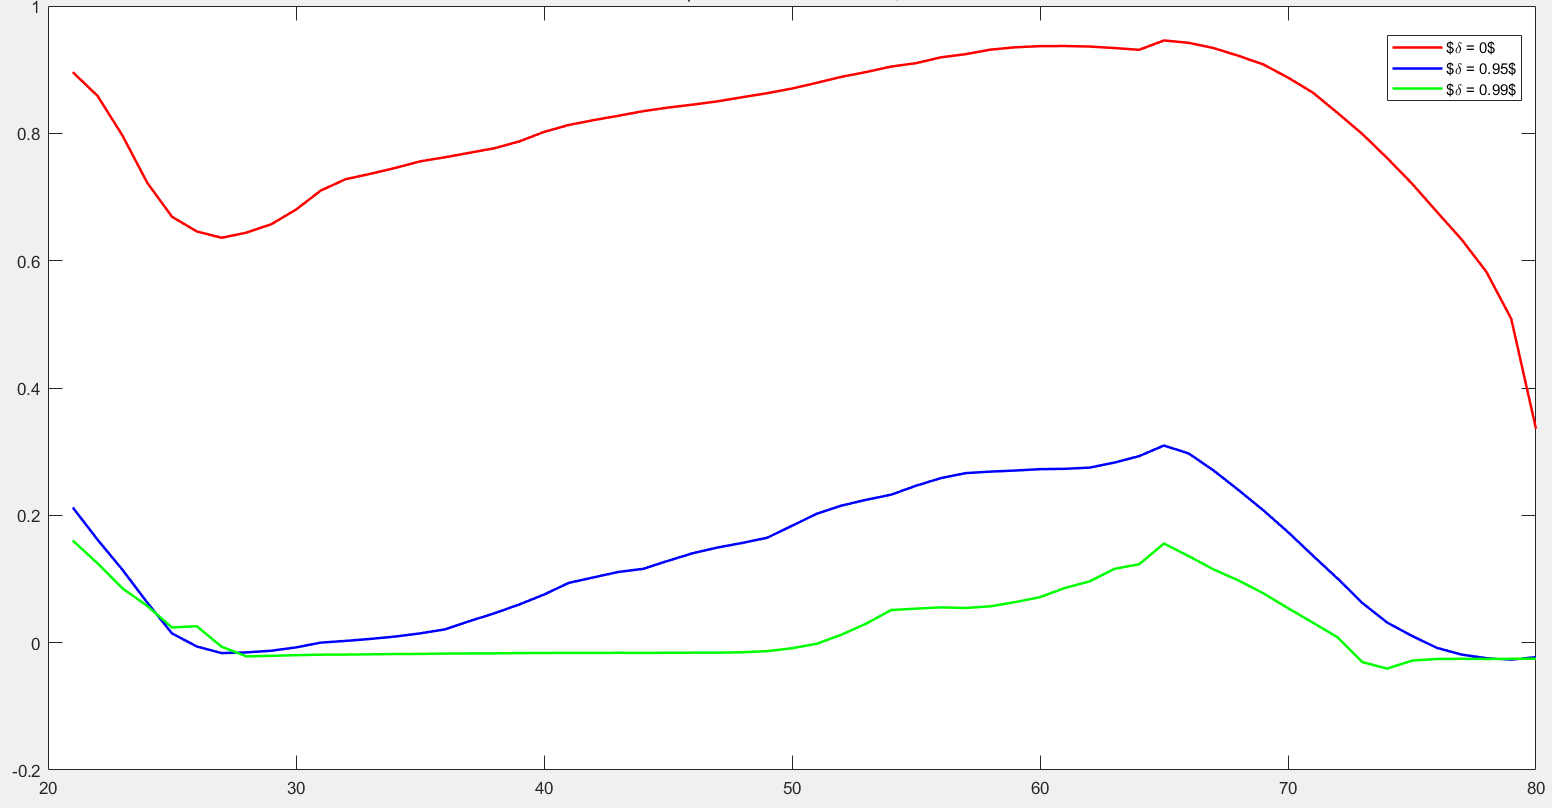
\includegraphics[width=10cm]{./figs/consinsurance}
\label{fig:conins}
\end{figure}


\section{General Equilibrium}

\end{document}
